\subsection{Experimental Methodology}
So far, we are able to collect whole-program execution traces, preprocess them (decompress, filter, detect loops, extract attributes) and inject each $PT$ to concept lattice data structure.
%
Concept lattices help us having a single model for the execution of HPC application with thousands of processes/threads.
%
Concept lattices also classify PTs based on their Jaccard distance.
%
Full pair-wise Jaccard distance matrix can be extracted from the concept lattice in linear time and reduces the search space from thousands of PTs to just a few equivalent classes of PTs.
%
Studying JSM by itself helps the user to understand the program behavior as a whole, and how each process/thread behaving.
%
However, comparing the JSM of the bug-free version of the application versus the buggy version would reveal insights about how the bug impacted the behavior of the application.
%
In particular, we are interested to see how the bug changes the formation of equivalent classes of PTs.
%
Inspired by a method for comparing two different clustering \cite{fowlkes83}, we count the number of objects (PTs) in each cluster and see which PT(s) fall into different clusters once the bug is introduced.
%
A set of candidate PTs then would be reported to the user for more in-depth study.
%
Here is where we take advantage of diffNLR to see how does the bug changes the control flow of a candidate PT comparing to its corresponding PT of native run.
%

\begin{figure*}[t]
\centering
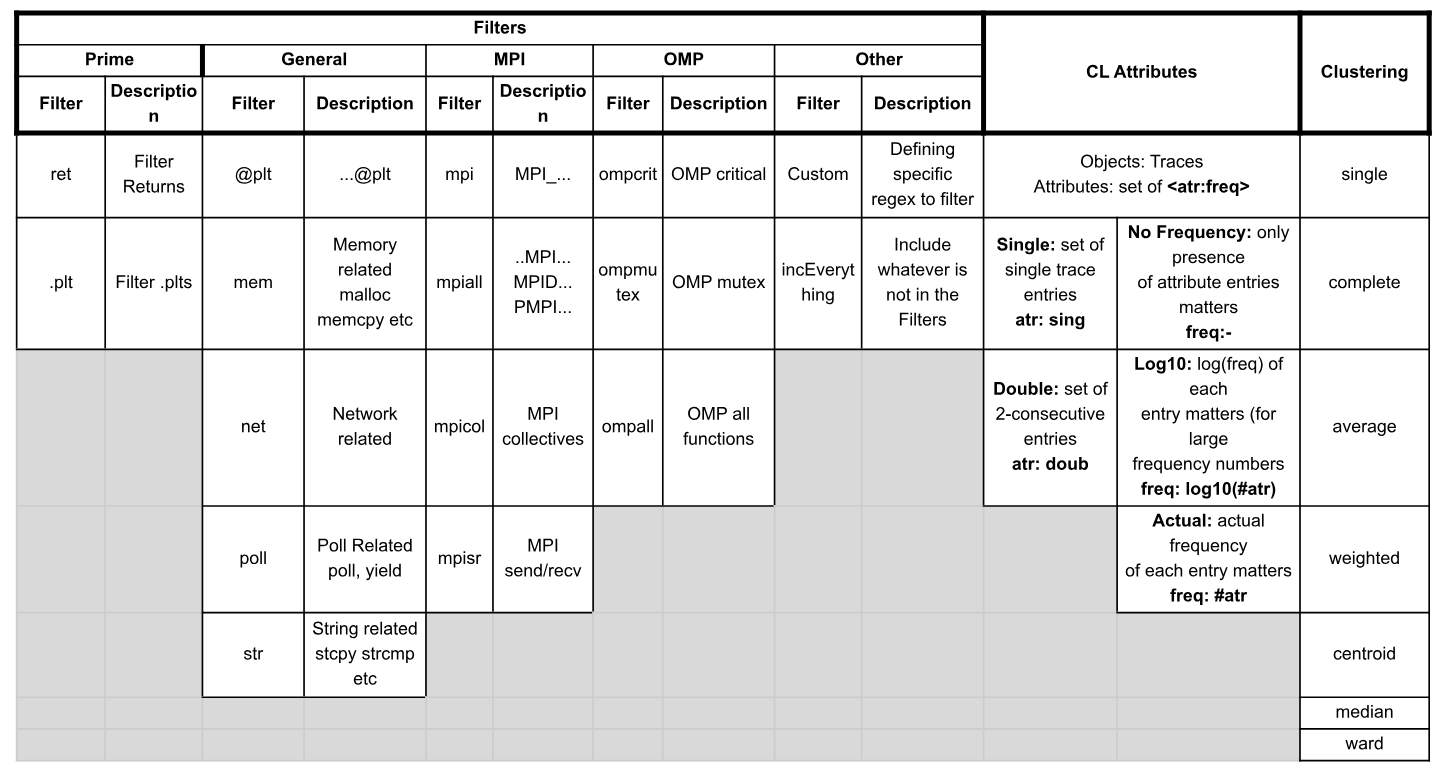
\includegraphics[width=6in]{figs/parametersTable.png}
\caption{Filters, Attributes and other Parameters used to pre-process ParLOT Traces (PTs)}
\label{tab:parameters}
\end{figure*}

Table \ref{tab:parameters} shows different parameters that we can pre-process PTs with. Each combination of these parameters would result in a different concept lattice, thus different JSM and different clusterings. 
%
A table similar to \ref{tab:bug1candidate} is created for each injected bug.
%
Each row of the table is showing the set of parameters used to create JSMs.
%
Then by calculating $ |JSM(buggy) - JSM(bugfree)| $ we are interested to see which PT changes the most after the bug injected and falls into a single cluster.
%
The object(s) in the cluster with the fewest members (below a threshold) are potential candidates of \textit{threads that are manifesting the bug} and the diff(buggy,bug-free) is in our interest to see how does the bug changes its control flow.

\subsection{Case Study: ILCS-TSP}
Here is the ILCS framework pseudo-code. User needs to write \texttt{CPU\_Init()},\texttt{CPU\_Exec()} and \texttt{CPU\_Output()}.
% ILCS Code for later references

\begin{frame}{}
  \lstset{language=C}
 \begin{lstlisting}
int main(argc,argv){
 MPI_Init();
 MPI_Comm_size()
 MPI_Comm_rank(my_rank)
 //Figuring local number of CPUs
 MPI_Reduce() // Figuring global number of CPUs
 CPU_Init();
 //For storing local champion results
 champ[CPUs] = malloc(); 
 MPI_Barrier();
 #pragma omp parallel num_threads(CPUs+1)
 {
  rank = omp_get_thread_num()
  if (rank == 0){ //communication thread
   do{
    //Find and report the thread with 
    //local champion, global champion
    MPI_AllReduce();
    //Find and report the process with
    //global champion
    MPI_AllReduce();	
    //The process with the global champion
    //copy its results to bcast_buffer	
    if (my_rank == global_champion){
     #pragma omp cirtical
     memcpy(bcast_buffer,local_champ)
    }
    //Broadcast the champion
    MPI_Bcast(bcast_buffer)
   } while (no_change_threshold);
   cont=0 // signal worker threads to stop
  } else{ // worker threads
   while(cont){
    //Calculate Seed
    local_result = CPU_Exec()
    if (local_result < champ[rank]){
     #pragma omp cirtical
     memcpy(champ[rank],local_result)
    }
   }
  }
 }
 //Find and report the thread with 
 //local champion, global champion
 MPI_AllReduce();
 //Find and report the process with 
 //global champion
 MPI_AllReduce();
 // The process with the global champion
 // copy its results to bcast_buffer	
 if (my_rank == global_champion){
  #pragma omp cirtical
  memcpy(bcast_buffer,local_champ)
 }
 //Broadcast the champion
 MPI_Bcast(bcast_buffer)
 if(my_rank==0){
  CPU_Output(champ)
 }
 MPI_Finalize()
}

/* User code for TSP problem */

CPU_Init(){
 // Read In data from cities
 // Calculate distances
 // Return data structure to store champion
}

CPU_Exec(){
 // Find local champions (TSP tours)
}

CPU_Output(){
 // Output champion
}


\end{lstlisting}
\end{frame}



Table \ref{tab.ilcsTspBugs} describes the bug that I injected to ILCS-TSP
\begin{table*}[t]
\caption{Injected Bugs to ILCS-TSP}
\label{tab.ilcsTspBugs}
\scalebox{0.9}{
\begin{tabular}{|c|c|l|l|}
\hline
ID & Level & \multicolumn{1}{c|}{Bugs} & \multicolumn{1}{c|}{Description} \\ \hline
1 & \multirow{8}{*}{MPI} & allRed1wrgOp-1-all-x & Different operation (MPI\_MAX) in only one process (buggyProc = 2) for MPI\_ALLREDUCE() in Line 21 \\ \cline{1-1} \cline{3-4} 
2 &  & allRed1wrgSize-1-all-x & Wrong size in only one process (buggyProc = 2) for MPI\_ALLREDUCE() in Line 21 \\ \cline{1-1} \cline{3-4} 
3 &  & allRed1wrgSize-all-all-x & Wrong Size in all processes for MPI\_ALLREDUCE() in Line 21 \\ \cline{1-1} \cline{3-4} 
4 &  & allRed2wrgOp-1-all-x & Different operation (MPI\_MAX) in only one (buggyProc) for first MPI\_ALLREDUCE() -- L277:ilcsTSP.c \\ \cline{1-1} \cline{3-4} 
5 &  & allRed2wrgSize-1-all-x & Wrong size in only one (buggyProc) for first MPI\_ALLREDUCE() -- L277:ilcsTSP.c \\ \cline{1-1} \cline{3-4} 
6 &  & allRed2wrgSize-all-all-x & Wrong Size in all processes for second MPI\_ALLREDUCE() -- L277:ilcsTSP.c \\ \cline{1-1} \cline{3-4} 
7 &  & bcastWrgSize-1-all-x & Wrong Size in only one (buggyProc) of MPI\_Bcast() -- L290:ilcsTSP.c \\ \cline{1-1} \cline{3-4} 
8 &  & bcastWrgSize-all-all-x & Wrong Size n all processes for MPI\_Bcast() -- L240:ilcsTSP.c \\ \hline
9 & \multirow{10}{*}{OMP} & misCrit-1-1-x & Missing Critical Section in buggyProc and buggyThread -- L170:ilcsTSP.c \\ \cline{1-1} \cline{3-4} 
10 &  & misCrit-all-1-x & Missing Critical Section in buggyThread  and all prcoesses -- L170:ilcsTSP.c \\ \cline{1-1} \cline{3-4} 
11 &  & misCrit-1-all-x & Missing Critical Section in buggyProc and all threads -- L170:ilcsTSP.c \\ \cline{1-1} \cline{3-4} 
12 &  & misCrit-all-all-x & Missing Critical Section in all procs and threads -- L170:ilcsTSP.c \\ \cline{1-1} \cline{3-4} 
13 &  & misCrit2-1-1-x & Missing Critical Section in buggyProc and buggyThread -- L230:ilcsTSP.c \\ \cline{1-1} \cline{3-4} 
14 &  & misCrit2-all-1-x & Missing Critical Section in buggyThread -- L230:ilcsTSP.c \\ \cline{1-1} \cline{3-4} 
15 &  & misCrit2-1-all-x & Missing Critical Section in buggyProc and all threads -- L230:ilcsTSP.c \\ \cline{1-1} \cline{3-4} 
16 &  & misCrit2-all-all-x & Missing Critical Section in all procs and threads -- L230:ilcsTSP.c \\ \cline{1-1} \cline{3-4} 
17 &  & misCrit3-1-all-x & Missing Critical Section in buggyProc and all threads -- L280:ilcsTSP.c \\ \cline{1-1} \cline{3-4} 
18 &  & misCrit3-all-all-x & Missing Critical Section in all procs and threads -- L280:ilcsTSP.c \\ \hline
19 & General & infLoop-1-1-1 & Injected an infinite loop after CPU\_EXEC() in buggyProc,buggyThread \& buggyIter L164:ilcsTSP.c \\ \hline
\end{tabular}
}
\end{table*}

\clearpage

\subsubsection{Bug1: Wrong Operation in MPI AllReduce()}
We have injected a bug (row 1 table \ref{tab:ilcsTspBugs}) where \texttt{MPI\_Allreduce()} had been invoked with a wrong operation in one of the processes ($P_{2}$)(\texttt{MPI\_MAX} instead of \texttt{MPI\_MIN}).
%

\textbf{::What is the runtime reaction to this bug:: Program terminated well without any error, crash, hang or throwing any exception. But the results might be corrupted. This might be a silent bug that diffTrace could reveal}

The last row of table \ref{tab:bug1candidate} is telling us that among all combinations of parameters (filters, attributes, etc.) PT 0 (ParLOT trace that belongs to thread 0 of process 0 got impacted the most after we inject the bug.
\begin{table}[t]
\caption{Bug 1: Wrong MPI operation in AllReduce() Candidate Table}
\label{tab:bug1candidate}
\scalebox{0.9}{
\begin{tabular}{|c|c|c|c|c|}
\hline
Filter & Attribute & \begin{tabular}[c]{@{}c@{}}K: \# of \\ diff Clusters\end{tabular} & \begin{tabular}[c]{@{}c@{}}\# Objects in each\\  Cluster (CL i)\end{tabular} & \begin{tabular}[c]{@{}c@{}}Candidate PT\\ Outliers\end{tabular} \\ \hline
 &  &  & CL 0:34 & - \\ \cline{4-5} 
\multirow{-2}{*}{11.mpi.cust.0K10} & \multirow{-2}{*}{sing.orig} & \multirow{-2}{*}{2} & CL 1:6 & - \\ \hline
 &  &  & CL 0:34 & - \\ \cline{4-5} 
 &  &  & CL 1:5 & \{2 3 4 27 29 \} \\ \cline{4-5} 
\multirow{-3}{*}{11.mpi.cust.0K10} & \multirow{-3}{*}{sing.orig} & \multirow{-3}{*}{3} & CL 2:1 & \{22 \} \\ \hline
 &  &  & CL 0:3 & \{24 38 39 \} \\ \cline{4-5} 
 &  &  & CL 1:31 & - \\ \cline{4-5} 
 &  &  & CL 2:5 & \{2 3 4 27 29 \} \\ \cline{4-5} 
\multirow{-4}{*}{11.mpi.cust.0K10} & \multirow{-4}{*}{sing.orig} & \multirow{-4}{*}{4} & CL 3:1 & \{22 \} \\ \hline
 &  &  & CL 0:34 & - \\ \cline{4-5} 
\multirow{-2}{*}{11.mpi.cust.0K10} & \multirow{-2}{*}{sing.log10} & \multirow{-2}{*}{2} & CL 1:6 & - \\ \hline
 &  &  & CL 0:34 & - \\ \cline{4-5} 
 &  &  & CL 1:5 & \{2 3 4 27 29 \} \\ \cline{4-5} 
\multirow{-3}{*}{11.mpi.cust.0K10} & \multirow{-3}{*}{sing.log10} & \multirow{-3}{*}{3} & CL 2:1 & \{22 \} \\ \hline
 &  &  & CL 0:3 & \{24 38 39 \} \\ \cline{4-5} 
 &  &  & CL 1:31 & - \\ \cline{4-5} 
 &  &  & CL 2:5 & \{2 3 4 27 29 \} \\ \cline{4-5} 
\multirow{-4}{*}{11.mpi.cust.0K10} & \multirow{-4}{*}{sing.log10} & \multirow{-4}{*}{4} & CL 3:1 & \{22 \} \\ \hline
 &  &  & CL 0:34 & - \\ \cline{4-5} 
\multirow{-2}{*}{11.mpi.cust.0K10} & \multirow{-2}{*}{sing.actual} & \multirow{-2}{*}{2} & CL 1:6 & - \\ \hline
 &  &  & CL 0:34 & - \\ \cline{4-5} 
 &  &  & CL 1:5 & \{2 3 4 27 29 \} \\ \cline{4-5} 
\multirow{-3}{*}{11.mpi.cust.0K10} & \multirow{-3}{*}{sing.actual} & \multirow{-3}{*}{3} & CL 2:1 & \{22 \} \\ \hline
 &  &  & CL 0:3 & \{24 38 39 \} \\ \cline{4-5} 
 &  &  & CL 1:31 & - \\ \cline{4-5} 
 &  &  & CL 2:5 & \{2 3 4 27 29 \} \\ \cline{4-5} 
\multirow{-4}{*}{11.mpi.cust.0K10} & \multirow{-4}{*}{sing.actual} & \multirow{-4}{*}{4} & CL 3:1 & \{22 \} \\ \hline
 &  &  & CL 0:39 & - \\ \cline{4-5} 
\multirow{-2}{*}{11.mpi.cust.0K10} & \multirow{-2}{*}{doub.orig} & \multirow{-2}{*}{2} & \textbf{CL 1:1} & \textbf{\{0\}} \\ \hline
 &  &  & CL 0:32 & - \\ \cline{4-5} 
 &  &  & CL 1:7 & - \\ \cline{4-5} 
\multirow{-3}{*}{11.mpi.cust.0K10} & \multirow{-3}{*}{doub.orig} & \multirow{-3}{*}{3} & \textbf{CL 2:1} & \textbf{\{0\}} \\ \hline
 &  &  & CL 0:32 & - \\ \cline{4-5} 
 &  &  & CL 1:7 & - \\ \cline{4-5} 
\multirow{-3}{*}{11.mpi.cust.0K10} & \multirow{-3}{*}{doub.orig} & \multirow{-3}{*}{4} & \textbf{CL 2:1} & \textbf{\{0\}} \\ \hline
 &  &  & CL 0:39 & - \\ \cline{4-5} 
\multirow{-2}{*}{11.mpi.cust.0K10} & \multirow{-2}{*}{doub.log10} & \multirow{-2}{*}{2} & \textbf{CL 1:1} & \textbf{\{0\}} \\ \hline
 &  &  & CL 0:32 & - \\ \cline{4-5} 
 &  &  & CL 1:7 & - \\ \cline{4-5} 
\multirow{-3}{*}{11.mpi.cust.0K10} & \multirow{-3}{*}{doub.log10} & \multirow{-3}{*}{3} & \textbf{CL 2:1} & \textbf{\{0\}} \\ \hline
 &  &  & CL 0:32 & - \\ \cline{4-5} 
 &  &  & CL 1:7 & - \\ \cline{4-5} 
\multirow{-3}{*}{11.mpi.cust.0K10} & \multirow{-3}{*}{doub.log10} & \multirow{-3}{*}{4} & \textbf{CL 2:1} & \textbf{\{0\}} \\ \hline
 &  &  & CL 0:39 & - \\ \cline{4-5} 
\multirow{-2}{*}{11.mpi.cust.0K10} & \multirow{-2}{*}{doub.actual} & \multirow{-2}{*}{2} & \textbf{CL 1:1} & \textbf{\{0\}} \\ \hline
 &  &  & CL 0:32 & - \\ \cline{4-5} 
 &  &  & CL 1:7 & - \\ \cline{4-5} 
\multirow{-3}{*}{11.mpi.cust.0K10} & \multirow{-3}{*}{doub.actual} & \multirow{-3}{*}{3} & \textbf{CL 2:1} & \textbf{\{0\}} \\ \hline
 &  &  & CL 0:32 & - \\ \cline{4-5} 
 &  &  & CL 1:7 & - \\ \cline{4-5} 
\multirow{-3}{*}{11.mpi.cust.0K10} & \multirow{-3}{*}{doub.actual} & \multirow{-3}{*}{4} & \textbf{CL 2:1} & \textbf{\{0\}} \\ \hline
\multicolumn{2}{|c|}{\cellcolor[HTML]{C0C0C0}{\color[HTML]{C0C0C0} }} & \textbf{\begin{tabular}[c]{@{}c@{}}TOP Suspicious\\ Traces to check\end{tabular}} & \textbf{\begin{tabular}[c]{@{}c@{}}1-0\\ 2-2\\ 3-3\end{tabular}} & - \\ \hline
\end{tabular}
}
\end{table}


\begin{figure}[t]
\centering
\scalebox{0.5}{
\includegraphics[width=6in]{figs/diffNLR/{bug1-1}.pdf}}
\caption{Bug1: diffNLR $PT_{0,0}$ - buggy vs. native}
\label{fig:bug1-1}
\end{figure}

The target MPI\_Allreduce() that we injected the bug to, finds the rank (i.e., process) that has the ``champion'' result among all of ranks using MPI\_MIN operator. Then that champion rank copies its ``champion results'' to a global data-structure and broadcast the ``champion results'' to all other ranks for the next time step.
However, since we changed the MPI\_MIN to MPI\_MAX in only one of the ranks, the true champion rank would get lost, instead a false champion rank (which turned to be rank 0 or $PT_{0,0}$) would broadcast its results as champion in the first time-step, causing a potential wrong answer. 
\clearpage


\subsubsection{Bug2: Wrong Size in MPI AllReduce() (one process)}
We have injected a bug (row 2 table \ref{tab:ilcsTspBugs}) where \texttt{MPI\_Allreduce()} had been invoked with a wrong size. \textbf{::MORE EXPLANATIONS ABOUT WHAT THE BUG IS::}
%

%\textbf{::What is the runtime reaction to this bug:: on node 3 (rank 3 in comm 0): Fatal error in PMPI\_Bcast: Invalid root}

Similar to table \ref{tab:bug1candidate}, the same ranking system tells us to check $PT_{1,0}$ and $PT_{3,0}$. Note that the bug injected to only one process ($P_3$) to have the wrong size.)

\begin{figure}[t]
\centering
\scalebox{0.5}{
\includegraphics[width=6in]{figs/diffNLR/{bug2-1}.pdf}}
\caption{Bug2: diffNLR $PT_{3,0}$ - buggy vs. native}
\label{fig:bug2-1}
\end{figure}


\begin{figure}[t]
\centering
\scalebox{0.5}{
\includegraphics[width=6in]{figs/diffNLR/{bug2-2}.pdf}}
\caption{Bug2: diffNLR $PT_{1,0}$ - buggy vs. native}
\label{fig:bug2-2}
\end{figure}


\textbf{::EXPLANATIONS OF OBSERVATIONS::}

\clearpage


\subsubsection{Bug3: Wrong Size in MPI AllReduce() (all processes)}
We have injected a bug (row 3 table \ref{tab:ilcsTspBugs}) where \texttt{MPI\_Allreduce()} had been invoked with a wrong size. \textbf{::MORE EXPLANATIONS ABOUT WHAT THE BUG IS::}
%

\textbf{::What is the runtime reaction to this bug:: on node 3 (rank 3 in comm 0): Fatal error in PMPI\_Bcast: Invalid root}

Similar to table \ref{tab:bug1candidate}, the same ranking system tells us to check $PT_{1,0}$ and $PT_{3,0}$. Note that the bug injected to only one process ($P_3$) to have the wrong size.)

\begin{figure}[t]
\centering
\scalebox{0.5}{
\includegraphics[width=6in]{figs/diffNLR/{bug2-1}.pdf}}
\caption{Bug2: diffNLR $PT_{3,0}$ - buggy vs. native}
\label{fig:bug2-1}
\end{figure}


\begin{figure}[t]
\centering
\scalebox{0.5}{
\includegraphics[width=6in]{figs/diffNLR/{bug2-2}.pdf}}
%\caption{Bug2: diffNLR $PT_{1,0}$ - buggy vs. native}
\label{fig:bug2-2}
\end{figure}


\textbf{::EXPLANATIONS OF OBSERVATIONS::}

\clearpage

\subsubsection{Bug4: Wrong Op in MPI AllReduce(): no effect!,program terminates fine}

maybe all images show some reflection

\subsubsection{Bug5: Wrong Size in next MPI AllReduce()(one process)::no effect, program terminates fine}

maybe all images show some reflection

\subsubsection{Bug6: Wrong Size in next MPI AllReduce()(all processes)::no effect,program terminates fine}

maybe all images show some reflection

\subsubsection{Bug7: Wrong Size in MPI Bcast()(one process)::}

maybe all images show some reflection

\subsubsection{Bug8: Wrong Size in next MPI Bcast()(all processes)::no effect,program terminates fine}

maybe all images show some reflection

\subsubsection{3: Missing Critical Section one thread in on process}

I planted the bug (missing critical section) in process 2

\begin{figure*}[t]
\centering
\includegraphics[width=6in]{figs/{miscrit-1-1-ranking}.png}
\caption{Part of ranking table for MisCrit 1-1}
\label{miscrit-1-1-rank}
\end{figure*}



\begin{figure*}[t]
\centering
\includegraphics[width=5.9in]{figs/{miscrit-1-1-1.3_2.3}.pdf}
\caption{diffNLR of process 1 thread 3 and process 2 thread 3 buggy(missing critical section) vs. bug-free}
\label{bug2.2}
\end{figure*}


